%# -*- coding: utf-8-unix -*-
%%==================================================
%% chapter01.tex for SJTU Master Thesis
%%==================================================

%\bibliographystyle{sjtu2}%[此处用于每章都生产参考文献]
\chapter{绪论}
\label{chap:intro}

大数据时代的到来和云计算的迅猛发展使得用分布式计算的方式来处理海量数据的方案变得水到渠成。
分布式并行计算框架的出现,特别是基于有向无环图(DAG)的方式来表达计算逻辑的分布式计算框架的出现,进一步简化了大数据处理的过程。
也因为分布式计算框架在处理大数据领域的重要性,使得其在短时间内获得了大量的普及。
虽然如何使得分布式计算变得更高效一直是近几年的研究热点,但是大量工作都集中在优化计算阶段的方向,而对于其中shuffle阶段则关注较少。
但不能忽视的是,在许多场景下,shuffle这种I/O密集型的操作会给分布式计算应用带来巨大的开销,甚至会成为整个分布式计算应用的性能瓶颈。

本文针对现有的分布式计算框架的shuffle特点,提炼出它们在shuffle过程中存在的共同问题,并据此提出了一种通用,高效的shuffle优化方案。
本章首先会介绍分布式计算框架的设计,相应的工作流程以及shuffle在其中的实现方式,然后阐述本文的优化目标以及国内外相关研究现状,最后简单介绍本文的结构组成。

\section{研究背景}

大数据时代的到来使得企业要处理的数据量远远超过了一台机器的处理性能。
在分布式计算普及之前,企业只能通过不断升级昂贵的超级计算机的性能来满足指数级增长的数据量。
然而随着Google公开了MapReduce\cite{mapreduce}的计算模式之后,分布式并行计算逐渐进入了蓬勃发展的阶段。
相对于昂贵而复杂的大型机,分布式计算能使用造价较低的商用机,并通过网络组合成集群,从而提供与超级计算机相匹配的运算能力来实现对大数据进行快速的批处理。
最近几年,更是有大量的分布式计算框架在学术界和工业界得以发表和公开。
同时也有大量的计算框架被部署到企业的生产环境中,成为大数据生态系统中最重要的一个组件。
其中应用最广泛的就是Hadoop MapReduce\cite{hadoop},Spark\cite{apachespark}和Tez\cite{tez}等。

虽然这些计算框架的设计和实现大相径庭,但是究其本质上对任务进行分布式并行处理的基本理念还是有着许多相似之处。

本节余下部分将首先介绍目前业界应用最广泛的以及学术界最具代表性分布式计算过框架的工作流程。
之后分析概况和归纳其在执行分布式任务中存在的共性,以此来说明本课题的研究存在普遍意义。

这些分布式计算框架中最经典的分布式计算框架便是Hadoop MapReduce\cite{hadoop}。
Hadoop MapReduce是根据Google发表的MapReduce\cite{mapreduce}论文修改并且开源而来。
其运行中的计算逻辑主要通过由用户定义具体的mapper和reducer来实现。
对于用户定义的mapper和reducer,Hadoop MapReduce会在执行过程中创建多个任务副本(Task)。
这些任务在任务调度器和资源调度器共同的调度下,会被分配到集群中的某个节点上的Java虚拟机(JVM)中进行执行。
而整个的MapReduce应用就是由这些mapper和reducer以及它们所对应的任务连接起来,形成一个流水线状的执行流程图。
具体可以参考图\ref{fig:mrdag}

\begin{figure}[!htp]
    \centering
    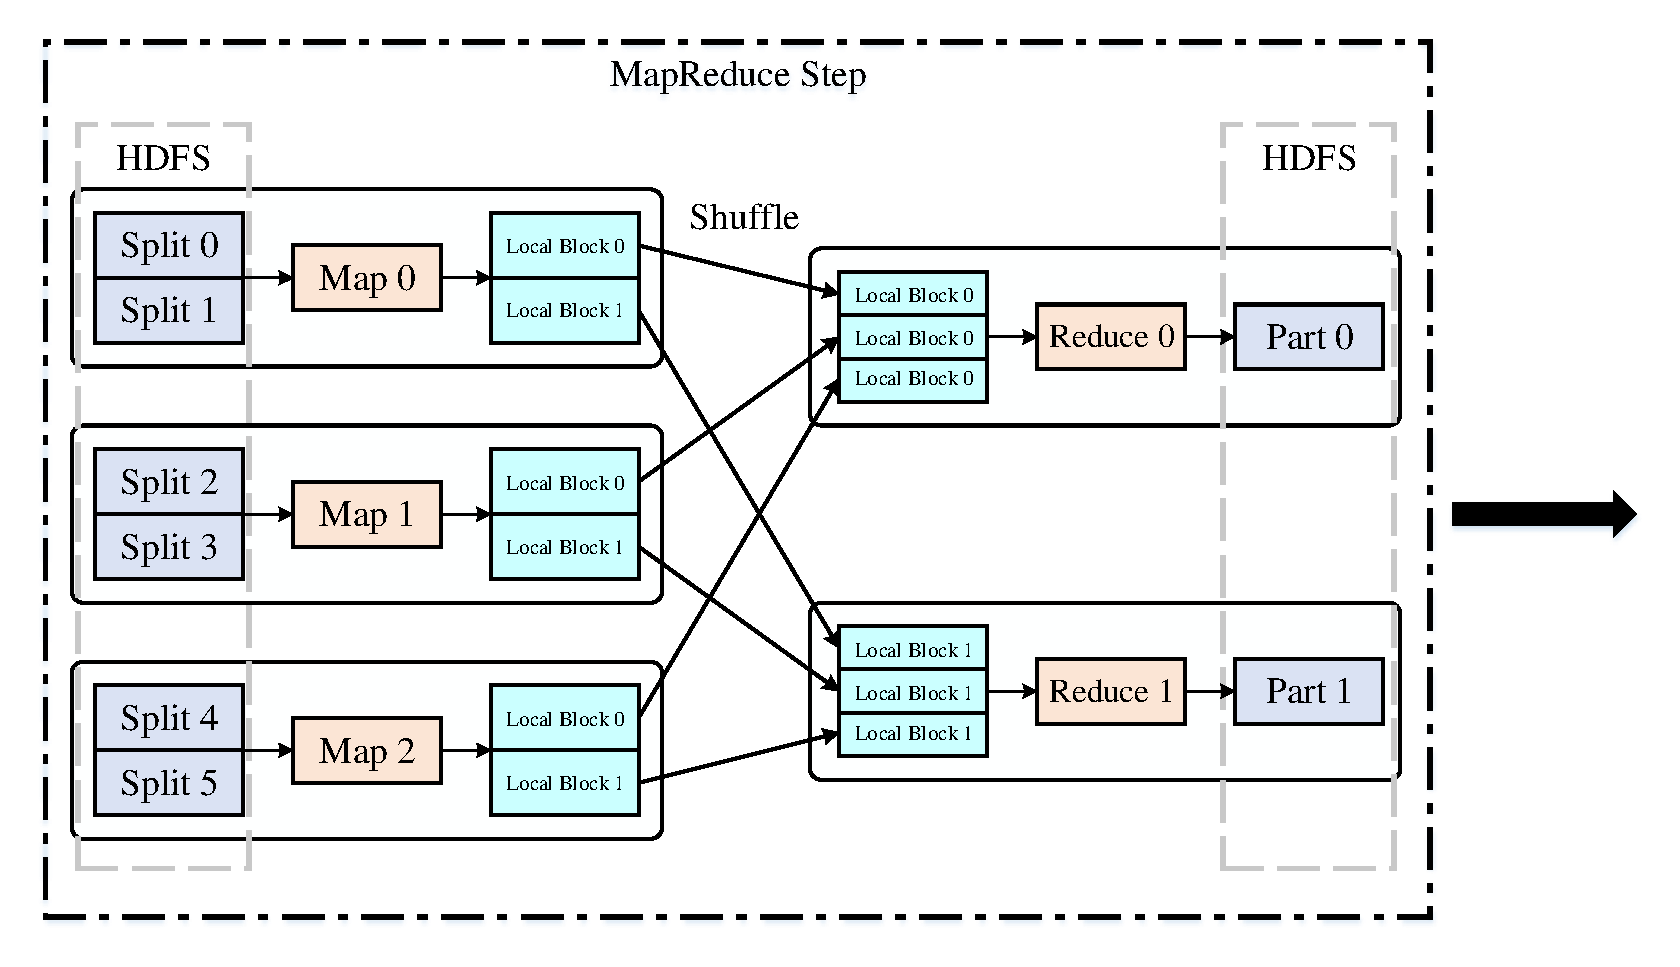
\includegraphics[width=0.9\textwidth]{mrdag.pdf}
	\bicaption[fig:mrdag]{Hadoop MapReduce执行示意图}{Hadoop MapReduce执行示意图}{Fig}{Hadoop MapReduce Execution Pipeline}
\end{figure}

在一个MapReduce应用开始时,其流水线的第一个任务会从分布式存储系统,比如HDFS中读取属于改任务的一部分数据。
之后在用户定义的mapper下对这部分数据进行操作,这部分称为map阶段。
在map阶段任务执行结束后,产生的中间结果会被保存到本地磁盘。
在map阶段所有任务执行结束之后,Hadoop MapReduce便会启动用户定义的reducer,开始reduce阶段的计算(此处不考虑slow-start)。
在reduce阶段的每个任务启动时,便会启动shuffle过程,即通过网络从远程节点的磁盘读取map阶段计算产生的中间结果。
当reduce阶段执行完成之后,产生的最终结果会被保存到分布式存储系统,为应用流水线的下一个步骤提供输入。
可以看到在经典的MapReduce计算过程中,每个reduce阶段结束之后多需要写入分布式存储系统,而且对于流水线中的map任务也存在大量的冗余操作。

Apache Tez\cite{tez}也是基于Hadoop的生态系统,在Yarn的基础上\cite{yarn}实现的分布式计算框架。
不同于MapReduce,Tez将原先的map和reduce操作拆分成了更细粒度的操作,并且通过顶点(vertex)和边(edge)的方式来表示运算逻辑,即DAG。
具体执行DAG可以参考图\ref{fig:tezdag}。
在Tez的DAG中,顶点代表了用户定义的运算逻辑,每个顶点中包含了具体的并行执行的运算任务,来实现分布式计算加速。
而边则表示顶点之间的数据依赖,从数据生产者指向消费者,其中三种比较常见的依赖为“一对一”,“广播”和“分散-聚合”(one-to-one, broadcast, scatter-gather)。
图\ref{fig:tezdag}中Vertex 1和Vertex 3之间的依赖便是“一对一”依赖,而剩下的则是“分散-聚合”依赖,也就是shuffle依赖。
在Tez执行DAG的过程中,每个reduce任务将不在进行对分布式存储系统的写入操作,从而避免了Hadoop MapReduce中reduce阶段完成后写入分布式系统的等待时间。
同时Tez也通过复用map任务的部分重复性操作,显著提高了运行效率。

\begin{figure}[!htp]
    \centering
    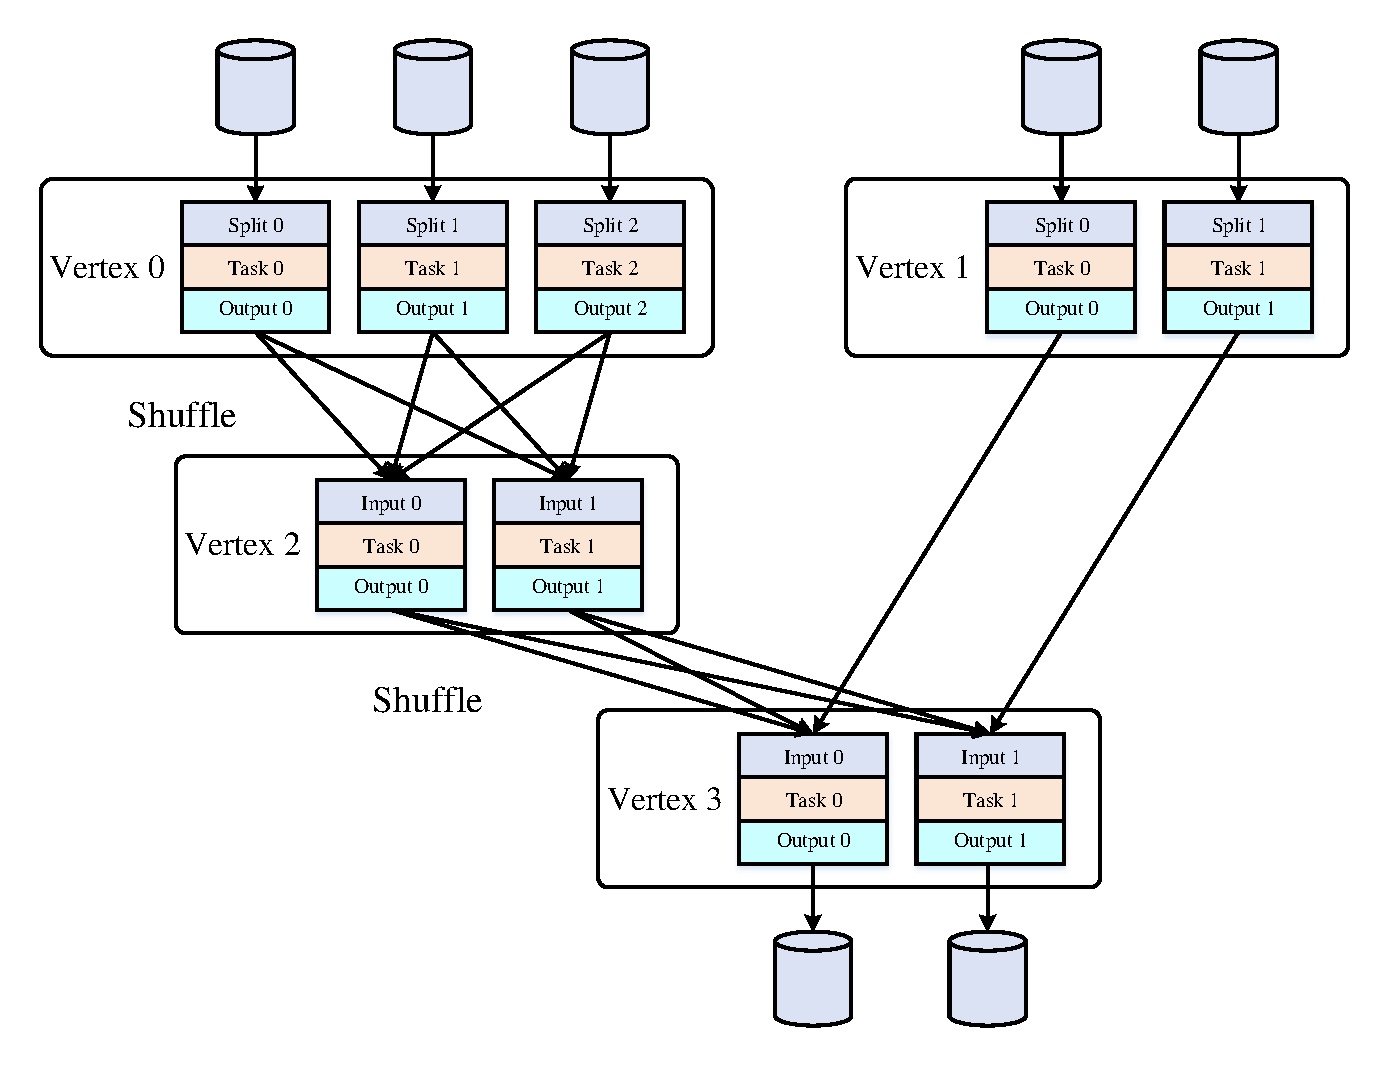
\includegraphics[width=0.9\textwidth]{tezdag.pdf}
	\bicaption[fig:tezdag]{Apache Tez执行示意图}{Apache Tez执行示意图}{Fig}{Execution DAG of Apache Tez}
\end{figure}

Spark\cite{spark}的出现和开源(Apache Spark\cite{apachespark})使分布式并行计算的效率和使用范围得到了进一步的提升。
在设计过程中,Spark为用户提供了丰富的接口(groupBy,union等),从而实现了更丰富的计算逻辑表达。
用户可以通过这些接口来对分布式应用进行编程设计。
在Spark的核心,用户的计算逻辑通过接口被翻译成了Resilient Distributed Datasets(RDD)之间的转换关系(transformation)。
连接RDD之间的转换关系最终在执行过程中行成系带(lineage),用来表示执行过程各个阶段之间的数据依赖。
在应用执行过程中,Spark采用了延迟绑定的策略,在执行时将这些依赖关系通过调度器优化成DAG,用来表达用户定义的计算过程。

图\ref{fig:sparkdag}展示了Spark在执行具体任务时的流程图。
Spark中的RDD在具体任务层面中与计算所需的分布式数据集一一对应。
其调度器会从用户提交的最后一个RDD开始延系带关系递归向前,当遇到转换关系中存在部分依赖时(partial dependency)便将其作为计算阶段(stage)的分界。
该递归过程会在寻找到已经计算完成的RDD或者该计算应用的最初始输入时停止。
对于一个节点上同一个阶段内的所有RDD之间的转换计算,Spark将其统一成一个任务(task),由其负责对该阶段内一个数据分区的所有运算。
同时,Spark会在任务执行时将RDD所对应的数据块缓存在节点内存中,从而使一个任务的所有转换计算都能在内存中高效得进行。
当分布式计算应用执行到部分依赖的时候,Spark会通过shuffle操作来满足下一个计算阶段的数据依赖。

\begin{figure}[!htp]
    \centering
    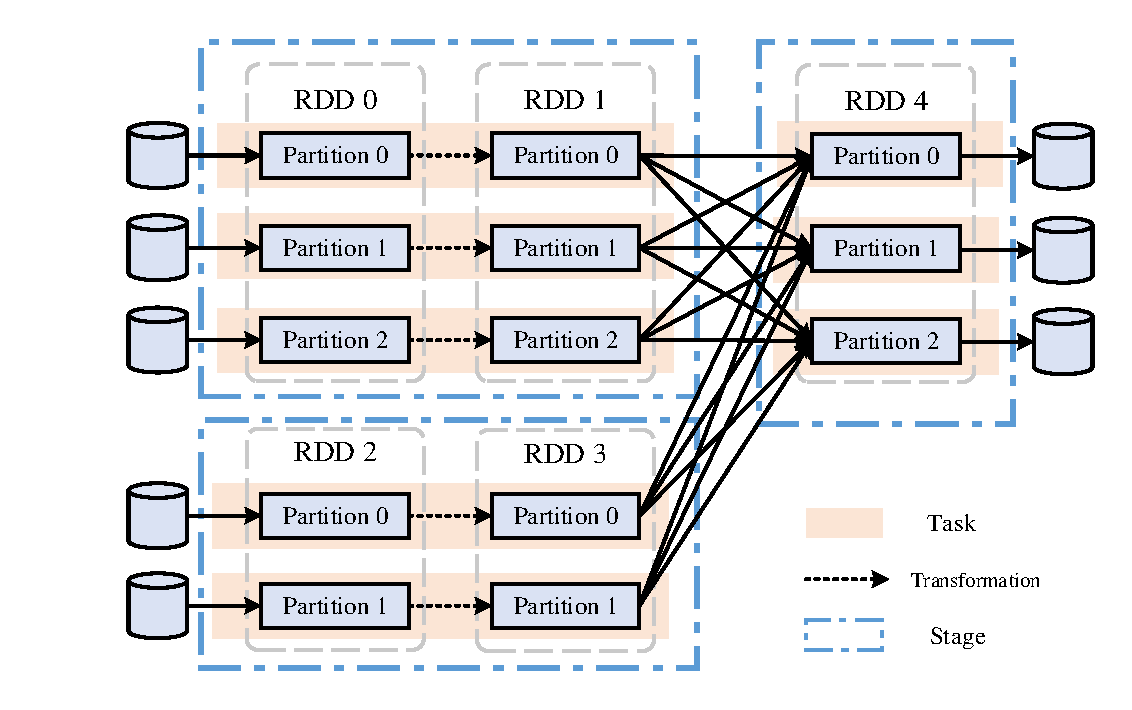
\includegraphics[width=0.8\textwidth]{sparkdag.pdf}
	\bicaption[fig:sparkdag]{Spark执行示意图}{Spark执行示意图}{Fig}{Execution DAG of Spark}
\end{figure}

在学术领域比较有代表性的一个分布式计算框架模型就是Dryad\cite{dryad}。
Dryad通过Nebula的脚本语言向用户提供接口。
用户可以通过该脚本语言来构造顶点和边,最终形成一个DAG。
其中顶点表示具体的某一种计算操作,每一条边则代表顶点之间的数据依赖模式。
具体数据的传递方式可以通过本地临时文件,TCP管道或者共享内存来实现。
临时文件是其实现数据流动的默认方式,在一个顶点的执行结束之后便会将运算结果输出到本地磁盘的临时文件。
TCP管道和共享内存都可以避免磁盘访问,但是TCP管道需要不同顶点同时运行,而共享内存甚至需要不同顶点在同一个进程里运行。

Dryad框架在获取用户提交的DAG之后,会将DAG划分成多个阶段(stage),每个阶段都包含了一个特定的计算顶点。
在Dryad执行具体应用时,会对相应的DAG进行运行时的优化。
比如对其中的多对一的和一对多的节点进行副本操作,从而增加计算过程的并发度。
经过优化之后的具体执行流程图如图\ref{fig:dryaddag}所示。
通过运行时优化之后,Dryad在执行过程中就会在每个计算阶段形成多个具有相同执行逻辑的顶点,而在采用默认的临时文件进行顶点间数据传输时,就会形成典型的shuffle传输。

\begin{figure}[!htp]
    \centering
    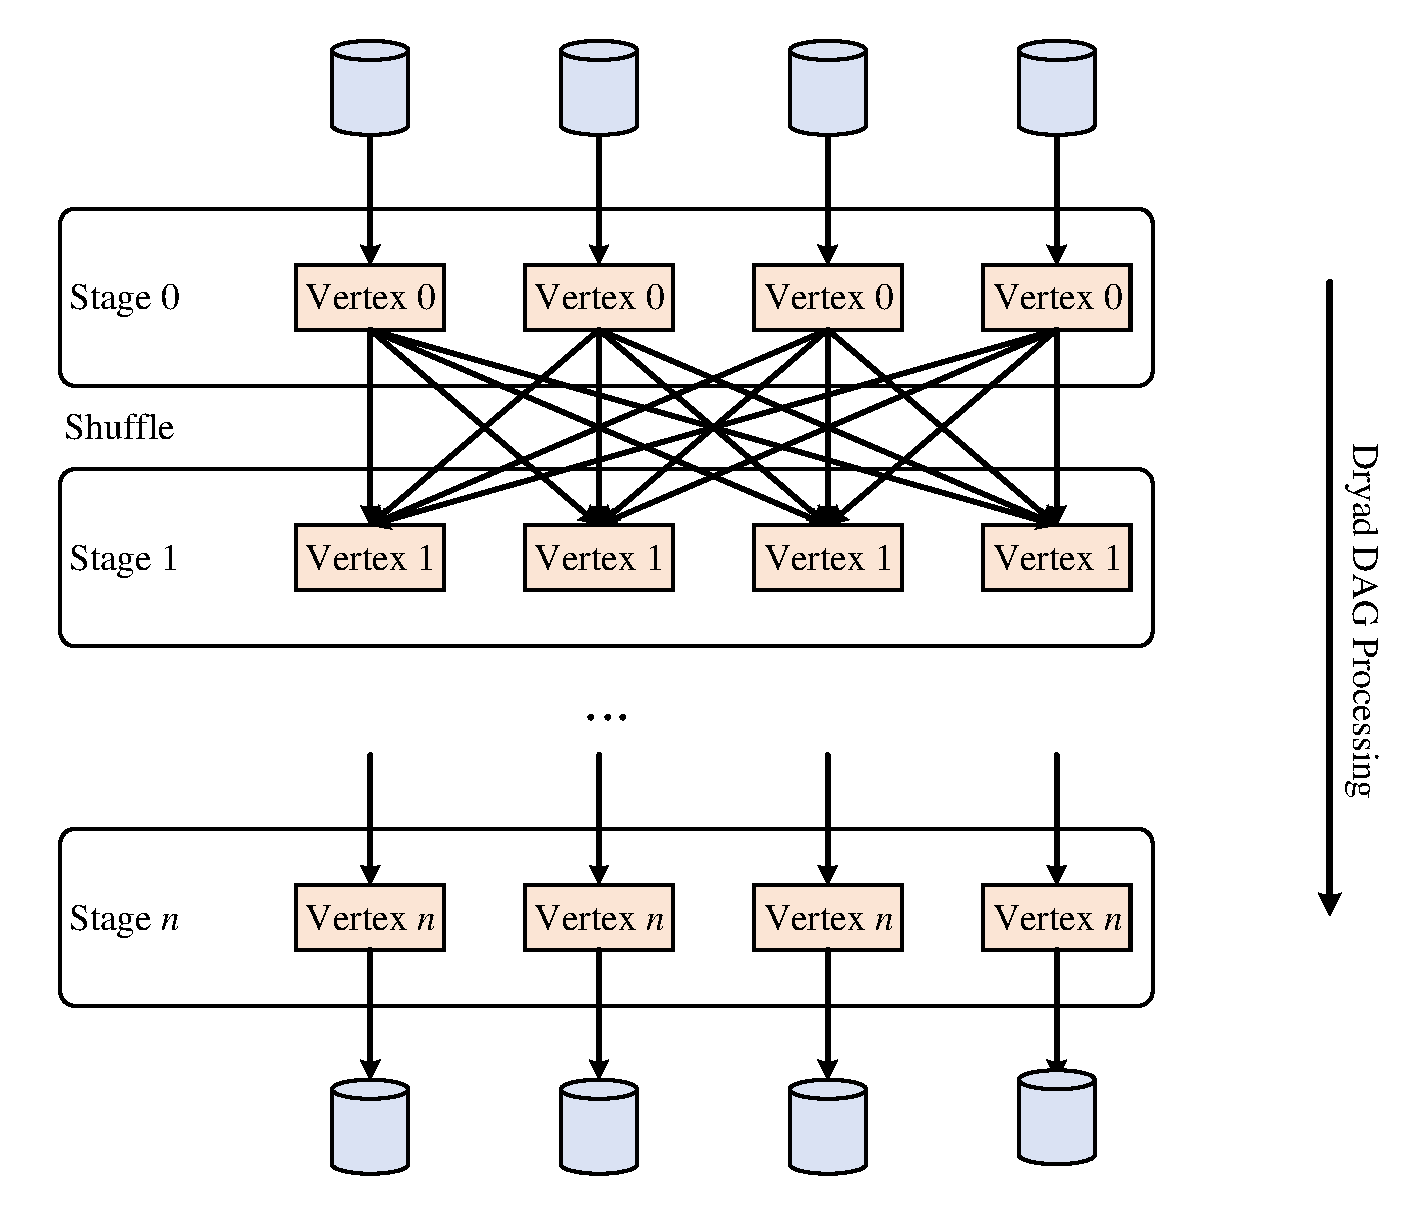
\includegraphics[width=0.8\textwidth]{dryaddag.pdf}
	\bicaption[fig:dryaddag]{Dryad执行示意图}{Dryad执行示意图}{Fig}{Execution DAG of Dryad}
\end{figure}

Pregel\cite{pregel}是主要针对于大规模图计算而设计的分布式图计算引擎。
其计算逻辑也由顶点和边构成的有向图。
但是值得注意的是Pregel的计算逻辑图是支持顶点间有环存在的。
Pregel中的每个顶点代表一个用户定义并且支持修改的状态。
而其中的有向边则连接了两个顶点,用来进行信息的传递。
其具体计算步骤则根据整体同步并行计算模型(Bulk Synchronize Parallel,BSP)来控制。
如图\ref{fig:pregel}所示,Pregel的执行过程由若干个superstep组成。
每个Superstep内的所有节点和虚线表示的有向边组合成表达用户计算逻辑的有向图。
其中每个边的方向则代表了一个superstep执行完成之后,节点之间数据流动的方向。
根部BSP模型,每个superstep会根据全局的同步信号来进行信息传递。
计算过程最终会在所有节点的算法都终止时结束。
在每个superstep内,执行图中的所有节点都会并发的进行本地的计算。
当完成一个superstep之后,每个节点都会根据定义的有向边向目的节点发送信息,之后进入下一步的计算。
而在superstep之间,需要完成一个多对多的顶点信息传输,也可以用shuffle来表示。

\begin{figure}[!htp]
    \centering
    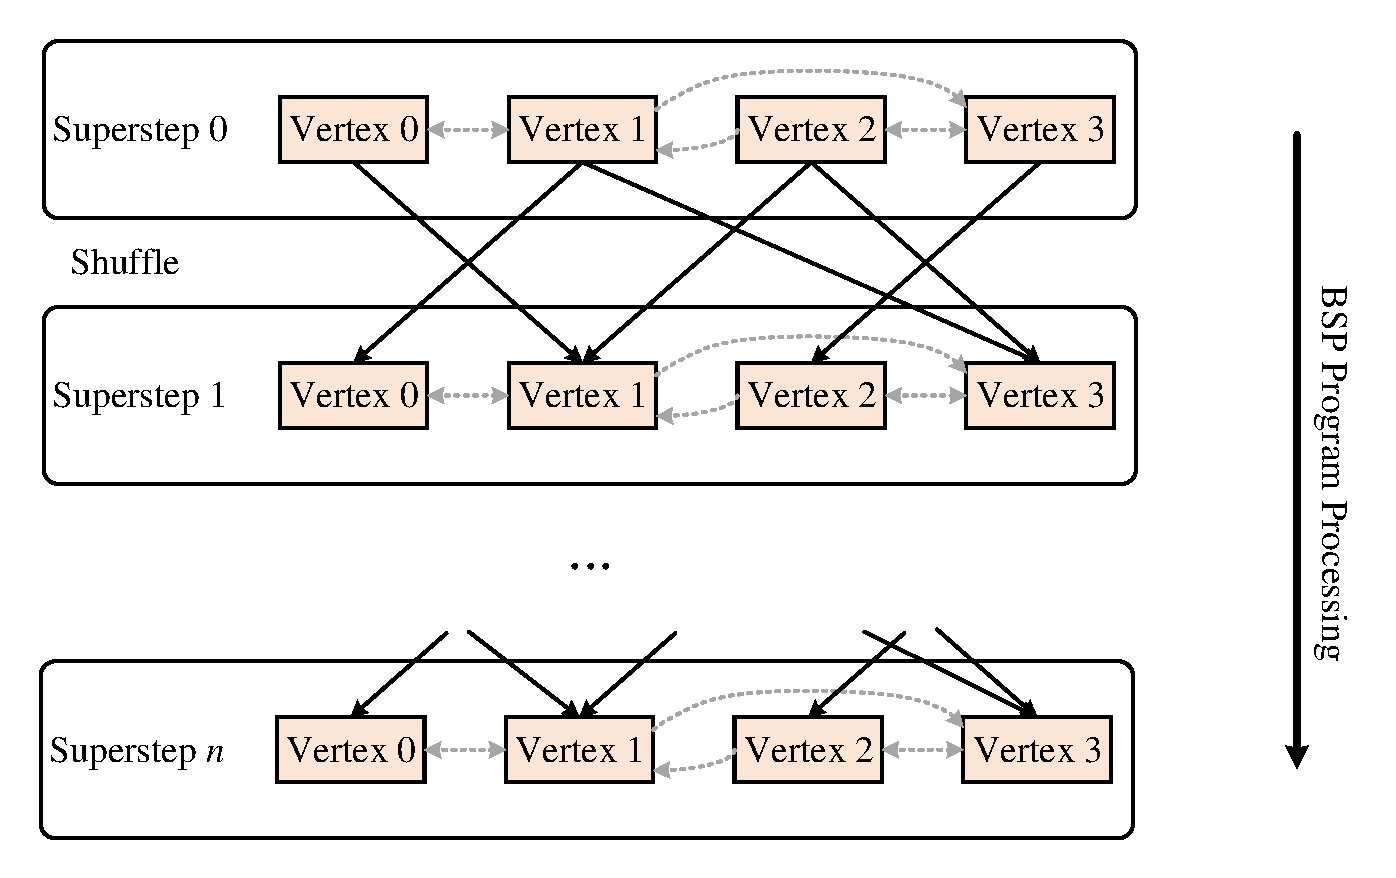
\includegraphics[width=0.8\textwidth]{pregel.pdf}
	\bicaption[fig:pregel]{Pregel执行示意图}{Pregel执行示意图}{Fig}{Execution Model of Pregel}
\end{figure}

综合对上述这些分布式计算框架的特点研究,我们发现虽然这些分布式计算框架的上层设计大相径庭,但是它们进行分布式任务执行的过程是十分相似的。
通过对上述这些框架的抽象概括,我们总结出一下几个共同点:

\begin{enumerate}
	\item 大部分计算框架都采用DAG来表达计算逻辑,即使如Pregel这种采用有向图的框架,其在计算过程中的BSP执行流程图也可以被看作是DAG。
	\item 在从执行逻辑到具体任务的转化过程中,这些计算框架都会采用一个任务多节点并行执行,每个任务处理一部分数据的方式,来提高分布式执行的效率。
	\item 在执行具体任务过程中,这些计算框架都采用类似BSP的模型来控制每个阶段的任务数据同步,比如Spark中的stage,Pregel中的superstep等。
	因此每个阶段之间都存在显示的屏障。
	\item 为了满足不同计算阶段之间,不同任务的数据依赖,这些计算框架都设计了不同方式的数据传输,而其中涉及到多对多的数据依赖时,其大都采用了本地磁盘缓存加网络传输的方式来进行实现。 
\end{enumerate}

\begin{figure}[!htp]
    \centering
    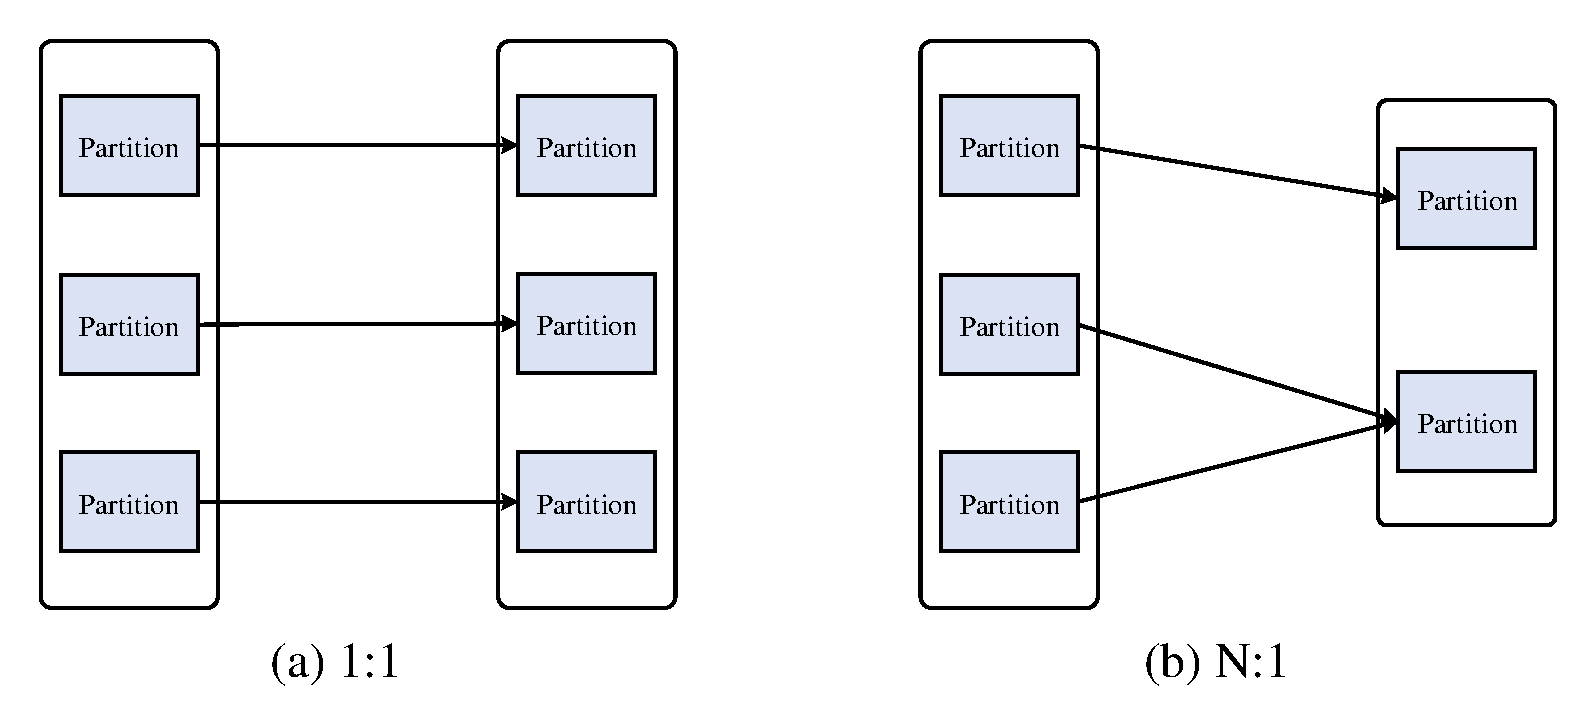
\includegraphics[width=0.8\textwidth]{narrowdep.pdf}
	\bicaption[fig:narrowdep]{完全依赖}{完全依赖}{Fig}{Full Dependency}
\end{figure}

总结归纳这些共同点,我们认为对于大部分分布式并行计算框架,其执行任务的本质就是在一个与计算逻辑有着对应关系的DAG中进行数据的处理和传输的过程。
其执行过程从数据流动的方向看,可以认为是被BSP模型的同步屏障显示的划分成的多个计算阶段的组合。
而在每个计算阶段的内部,从数据分块的方向看,其在执行时同时存在若干并行的任务,在集群不同的节点上对每个数据块进行计算。
所以,为了满足每个计算阶段内部不同任务对数据的依赖,在各个计算阶段之间存在着不同的依赖关系,反应到DAG中,则是不同模式的有向边组合。
这些数据依赖模式从DAG顶点与有向边对应关系的角度,可以分为“一对一”,“一对多”,“多对一”和“多对多”。
而从计算任务本身对数据的依赖角度,我们可以将这种对应关系更精简的分为两类:完全依赖和部分依赖。

图\ref{fig:narrowdep}中(a)和(b)均表示是完全依赖,即当前计算阶段中一个任务所需要的输入数据完全依赖于上一个计算阶段的一个或几个任务的所有输出数据。
反应在DAG执行图中边的形态,就是“一对一”或者“多对一”的情况。
对于完全依赖,由于一个任务依赖于是上一计算阶段任务输出的若干个完整的数据块,从而可以避免该任务对上一阶段剩余部分数据块计算结果的依赖,因此比较容易优化,而且目前业界已经有了比较成熟的方案。
比如Spark通过利用数据的完全依赖性,将DAG计算过程中连续的完全依赖打包成一个计算阶段(stage)。
同时,对于完全依赖中的每一个完整的数据块的运算过程打包成一个任务(task)。
在调度任务的过程中,通过内存缓存机制使DAG中完全依赖的这部分计算过程在本地节点的内存中连续进行,从而实现加速DAG执行过程。

部分依赖则表示当前计算阶段的一个任务所需要的输入数据依赖于上一个计算阶段的多个任务的部分数据,如图\ref{fig:widedep}所示。
反应在DAG执行图中,则可以是“一对多”或者“多对多”的形态,其中“多对多”本质上则是多个“一对多”的组合。
这种部分依赖在DAG中行程的点与边的数据传输过程通常称之为shuffle。

\begin{figure}[!htp]
    \centering
    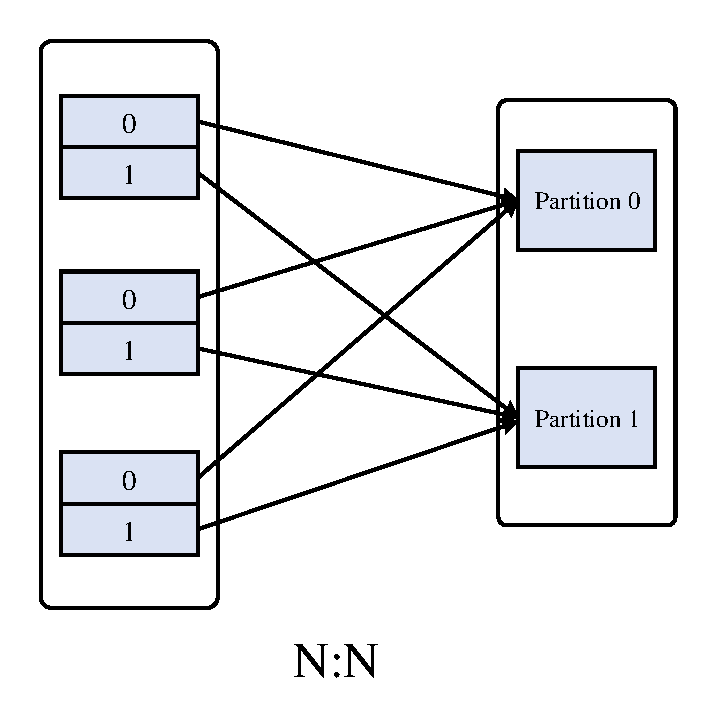
\includegraphics[width=0.4\textwidth]{widedep.pdf}
	\bicaption[fig:widedep]{部分依赖}{部分依赖}{Fig}{Partial Dependency}
\end{figure}

为了下文方便描述,这里我们对于具有以上特征的分布式计算框架统称为分布式DAG计算框架,简称为DAG计算框架。
对于DAG计算过程中,产生shuffle数据的一端,我们称之为map阶段(Map Stage),而对于接收shuffle数据的一端,我们称之为reduce阶段(Reduce Stage)。
虽然这些分布式计算框架在设计上存在很多不同,但是由于这种依赖的特殊性,需要依赖整个计算数据集中所有分区的部分数据,因此必须通过网络传输来满足数据在分布式系统中的传递。
所以分布式计算框架在处理部分依赖时大都采用了相似的策略,即通过本地磁盘来缓存map阶段的计算结果,等该map阶段所有任务执行完成之后,通过网络来实现数据多对多的传输。
因此shuffle阶段不可避免的需要通过速度相对较慢的I/O设备来完成。
而由于受限于I/O设备的性能(磁盘,网络等),shuffle很可能会对整个端到端的应用执行带来很大的额外开销。

虽然近几年针对分布式DAG计算框架的计算阶段学术界和企业界都提出了很多优化方案\cite{pacman, babu, quincy, sync},但是对于shuffle阶段在实际应用中的优化却一直很不理想。
比如在Facebook公开的一个MapReduce运行数据分析中,shuffle平均占到了所有任务完成时间的33\%。
对于需要大量shuffle的一些任务,shuffle的开销最多可以占到整个任务完成时间的70\%\cite{managing}。



\section{研究内容}

本文首先通过对这些DAG计算框架中部分开源产品的研究,发现制约shuffle性能的主要是由于缺乏对于不同类型的硬件资源的细粒度的管理和调度,以及在BSP计算模型下计算阶段之间的同步机制引起的低效率网络传输造成的。
在目前的DAG计算框架调度算法中,对于一个计算阶段的每一个任务,DAG计算框架的调度器都会分配集群中一部分固定的硬件资源,包括CPU,内存,磁盘和网络等。
为了简化调度算法,这些资源被捆绑成一个资源槽(slot)来进行粗粒度的管理和分配。
这种粗粒度的调度算法虽然简化了任务调度过程,但是也引入无法充分利用硬件资源的问题。
比如,当一个任务进行CPU内存密集的数据计算时,该slot所占用的I/O资源就会被闲置。
反之,当任务进行I/O密集的shuffle过程时,CPU和内存等计算资源就会被闲置。

除此之外,在shuffle阶段不可避免得会引入多对多的网络数据传输。
在目前的分布式DAG计算框架中,此阶段的网络数据传输也没有得到很好的管理。
受限于BSP模型的同步机制,一个计算阶段需要等到其所有任务完成,在此之后下一个阶段的任务才能开始被调度并且读取数据。
对于shuffle的两端,当map阶段的任务结束之后,大部分计算框架都选择用本地磁盘来保存计算结果,并且等待同步信号。
当reduce阶段被调度并启动之后,集群中会有多个reduce任务同时启动,与此同时,reduce任务会通过网络远程读取磁盘的操作来满足每个任务对map阶段输出数据的依赖。
而更重要的是,这个过程会在每个reduce任务的初始阶段几乎同时开始。
这种几乎同步的数据传输模式会给集群的网络带来一个瞬时的流量高峰。
而当带宽有限的情况下,这种瞬时的高峰极易造成网络的拥塞,从而进一步减慢了数据传输的速率。

更糟糕的是,上述发现的问题存在于大部分主流的分布式计算框架当中。
所以仅仅只是针对其中某一个框架提出解决方案并不能很好的缓解shuffle给分布式计算带来的性能开销。

为了给shuffle过程提供一个具有普适性的优化方案,本文提出了S(huffle)Cache --- 一个开源的即插型shuffle管理系统,给不同的DAG计算框架提供高效的shuffle管理和优化。
具体来说,SCache通过提供跨框架的API设计,来接管在DAG计算过程中的shuffle阶段。
同时SCache采用了以下几点关键创新,来实现对于shuffle的高效管理和优化:

\begin{enumerate}
	\item 将shuffle从计算过程中的解耦。使得shuffle的过程独立到DAG计算框架外部进行管理,从而实现了更细粒度的硬件资源管理,提高硬件资源的复用率和利用率,进而加速shuffle过程。
	\item 结合应用的上下文对reduce任务进行预调度。采取了启发式算法,根据map阶段执行过程中间状态,结合应用的上下文逻辑和数据本地性等特征提前调度reduce阶段的任务。
	\item 对shuffle数据进行预取。在map执行阶段,根据启发式预调度算法的结果,对shuffle数据进行预取,既避免了同步数据读取给网络带来的压力,又能将大部分网络传输时间隐藏到计算的阶段。
	\item 采用了结合上下文的内存管理机制。根据DAG计算框架的任务调度策略,对不同的shuffle数据块设置优先级,同时提前将shuffle数据缓存在内存当中,加速shuffle数据的读取过程,提升任务计算性能。
	\item 设计了具有普适性的API。SCache不仅根据shuffle的读写为DAG计算框架设计了相应的API,同时也为DAG框架的调度器设计了相应提交shuffle相关元数据和获取预调度结果的API。
\end{enumerate}

\section{国内外研究现状}
\label{sec:relatedwork}

目前国内外的对shuffle的优化工作主要分成三个方向:提前调度,延迟调度和纯网络层面的优化。

\textbf{提前调度}:Slow-start作为Hadoop MapReduce\cite{hadoop}中最经典的shuffle优化,是提前调度的代表性方案。
Starfish\cite{starfish}通过对数据的采样来自动调整MapReduce中的系统参数,比如slow-start的比例,map和reduce任务的比例等待。
DynMR\cite{dynmr}通过动态的在map阶段末端启动reduce任务来减少对与shuffle数据的等待。
以上所有这些方案都没有将I/O操作从计算密集型的任务中解耦,因而仍然在slot中留下显示的I/O等待时间。
而且由于计算资源有限,提前启动reduce任务会占用有限的slot,减慢map阶段的执行。
所以在设定何时启动提前调度的参数时,会受到应用,输入数据,当前硬件资源等条件的影响,不仅参数设置困难,优化效果也会有较大波动。
iShuffle\cite{ishuffle}采用了将shuffle从reduce阶段解耦的方式,并且提供了一个中心控制器来调度shuffle。
但是这个方案并不能很好的处理对多个shuffle的依赖。
iHadoop\cite{ihadoop}采用了激进地提前调度多个接下来的计算阶段的任务,从而使得shuffle数据的预取成为可能。
Drizzle\cite{drizzle}也采用了提前调度任务的方式来实现shuffle数据的预取。
但是在我们研究过程中发现,随机激进地调度任务可能会破坏DAG计算框架的负载均衡,从而减慢分布式应用的执行速度。

\textbf{延迟调度}:Delay Scheduling\cite{delay}采用延迟分配任务来获取更好的数据本地性,进而减少了shuffle阶段的网络数据传输。
ShuffleWatcher\cite{shufflewatcher}会在网络将近饱和的时候延迟shuffle数据的获取。同时它能在调度任务时获取更好的本地行。
Quincy\cite{quincy}和Fair Scheduling\cite{preemptive}都可以通过优化map任务的调度来获取更好的shuffle数据本地性。
但是以上这些工作都不能消除在计算任务中显示的I/O操作。更重要的是,他们的优化效果会因为网络的性能好坏和计算数据的不同分布而产生波动。

\textbf{网络层优化}:Varys\cite{varys},Aalo\cite{aalo},CODA\cite{coda},Seagull\cite{seagull}都能结合应用层信息提供shuffle在网络传输时的优化,从而加快shuffle的传输过程。
而DCTCP\cite{dctcp},pFabric\cite{pfabric},Pias\cite{pias},CONGA\cite{conga}等工作能结合数据中心网络的特点在纯网络层降低网络流的平均完成时间,增加网络吞吐。
虽然这些优化仅仅局限在shuffle过程中的网络传输部分,但是它们可以为本研究的优化提供进一步的性能提升。
比如本文在进一步优化shuffle的网络传输过程中,采用了Coflow\cite{coflow}的接口和Seagull的调度策略,给shuffle传输提供进一步的优化。

\section{文章结构}

本文余下内容结构如下:

第二章介绍shuffle在分布式并行DAG计算框架中的特点以及相关背景。通过对shuffle特性的分析,来挖掘其可优化的空间和制定具体优化方案。

第三章详细介绍了SCache的具体设计与实现,包括SCache的架构,shuffle调度算法设计,接口设计,内存管理策略以及网络层进一步优化等。
同时还会结合Spark\cite{apachespark}和Hadoop MapReduce\cite{hadoop}探讨SCache优化方案的普适性。

第四章对SCache在Spark\cite{apachespark}平台上的优化效果进行了实验和分析。
通过仿真实验和Amazon AWS EC2上虚拟机集群的测试,验证了SCache在shuffle上的优化效果。

第五章对全文进行了总结,并且对未来的工作方向做出展望。







